\documentclass[12pt]{article}
\usepackage{graphicx} 
\usepackage[margin=2cm]{geometry}
\usepackage[cmex10]{amsmath}
\usepackage{gensymb}
\usepackage{siunitx}
\usepackage{array}
\usepackage{float}
\usepackage{gvv-book}
\usepackage{gvv}


\title{Geomatics Engineering (2024)}
\author{Aditya Appana}
\date{August 2025}

\begin{document}

\maketitle

\section*{\underline{General Aptitude (GA)}}


\begin{enumerate} 

\item If ‘→’ denotes increasing order of intensity, then the meaning of the words [smile → giggle → laugh] is analogous to [disapprove → \rule{1.5cm}{0.15mm} → chide]. Which one of the given options is appropriate to fill the blank?


 \begin{enumerate}
   \begin{multicols}{4}
 

   \item reprove  
   \item praise  
   \item reprise  
   \item grieve  
\end{multicols}
\end{enumerate}

\item Find the odd one out in the set: \cbrak{19, 37, 21, 17, 23, 29, 31, 11}

\begin{enumerate}
\begin{multicols}{4}

    \item 21  
   \item 29  
   \item 37  
   \item 23  
 \end{multicols}  
\end{enumerate}

\item In the following series, identify the number that needs to be changed to form the
Fibonacci series. 1, 1, 2, 3, 6, 8, 13, 21  

\begin{enumerate}
\begin{multicols}{4}

    \item8 
   \item 21 
   \item 6  
   \item 13 
   \end{multicols}
\end{enumerate}


\item The real variables $x,y,z$ and the real constants $p,q,r$ satisfy  \\   \begin{Large} $\frac{x}{pq-r^2}$ =     $\frac{y}{qr-p^2}$ = $\frac{z}{rp-q^2}$ \end{Large}

\begin{enumerate}
\begin{multicols}{4}

    \item0  
   \item 1  
   \item $pqr$  
   \item $p^2 + q^2 + r^2$   
 \end{multicols}
\end{enumerate}

\item Take two long dice (rectangular parallelepiped), each having four rectangular faces
labelled as 2, 3, 5, and 7. If thrown, the long dice cannot land on the square faces
and has 1/4 probability of landing on any of the four rectangular faces. The label on
the top face of the dice is the score of the throw.

If thrown together, what is the probability of getting the sum of the two long dice
scores greater than 11? 

\begin{enumerate}  
\begin{multicols}{4}


    \item3/8 
   \item 1/8 
   \item 1/16  
   \item 3/16
   \end{multicols}
 \end{enumerate}

\item In the given text, the blanks are numbered (i)---(iv). Select the best match for all the
blanks.

Prof. P \rule{0.5cm}{0.15mm}(i)\rule{0.5cm}{0.15mm} merely a man who narrated funny stories. \rule{0.5cm}{0.15mm}(ii)\rule{0.5cm}{0.15mm} in his blackest moments he was capable of self-deprecating humor.

Prof. Q \rule{0.5cm}{0.15mm}(iii)\rule{0.5cm}{0.15mm} a man who hardly narrated funny stories. \rule{0.5cm}{0.15mm}(iv)\rule{0.5cm}{0.15mm} in his blackest moments was he able to find humor.

\begin{enumerate}
   

\item (i) was (ii) Only (iii) wasn’t (iv) Even  
   \item (i) wasn't (ii) Even (iii) was (iv) Only 
   \item (i) was (ii) Even (iii) wasn't (iv) Only  
   \item (i) wasn't (ii) Only (iii) was (iv) Even 
    
\end{enumerate}

\item How many combinations of non-null sets A, B, C are possible from the subsets of
{2, 3, 5} satisfying the conditions: (i) A is a subset of B, and (ii) B is a subset of C?  

\begin{enumerate}
\begin{multicols}{4}

     \item28 
   \item 27 
   \item 18  
   \item 19 
   \end{multicols}
\end{enumerate}


\item The bar chart gives the batting averages of VK and RS for 11 calendar years from
2012 to 2022. Considering that 2015 and 2019 are world cup years, which one of
the following options is true?

\begin{figure}[H]
\centering
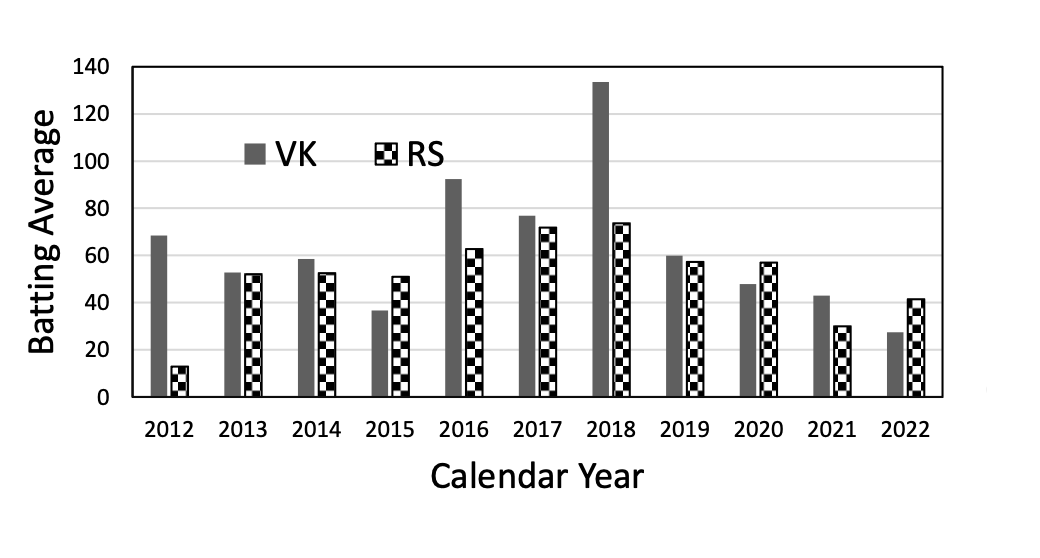
\includegraphics[width=0.5\columnwidth]{Figs/LatexGraph.png}
\caption{Batting Average vs Calendar Year}
    \end{figure}

\begin{enumerate}
     \item RS has a higher yearly batting average than that of VK in every world cup year.  
   \item VK has a higher yearly batting average than that of RS in every world cup year. 
   \item VK’s yearly batting average is consistently higher than that of RS between the two
world cup years.  
   \item  RS’s yearly batting average is consistently higher than that of VK in the last three
years. 
\end{enumerate}



\item A planar rectangular paper has two V-shaped pieces attached as shown below.
\begin{figure}[H]
\centering
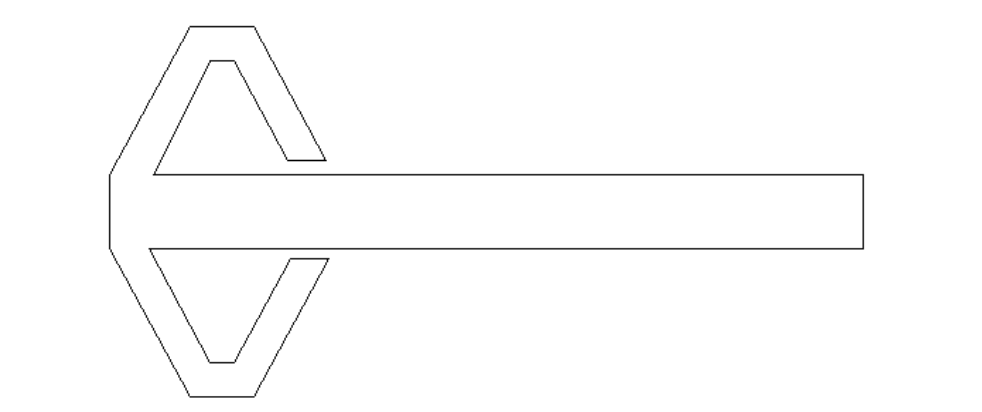
\includegraphics[width=0.5\columnwidth]{Figs/LatexImage1.png}
\end{figure}

This piece of paper is folded to make the following closed three-dimensional object.

\begin{figure}[H]
\centering
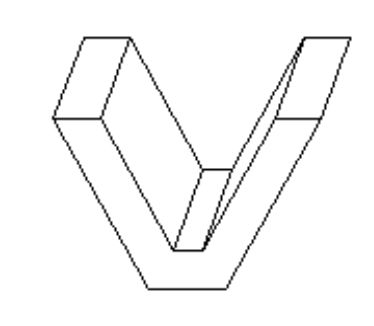
\includegraphics[width=0.5\columnwidth]{Figs/LatexImage2.png}
\end{figure}


 \begin{enumerate}
 \begin{multicols}{4}

    \item 9 
   \item 7 
   \item 11  
   \item  18
   \end{multicols}
 \end{enumerate}


\item  Four equilateral triangles are used to form a regular closed three-dimensional object
by joining along the edges. The angle between any two faces is 
\begin{enumerate}
\begin{multicols}{4}

    \item 30\degree 
   \item 60\degree 
   \item 45\degree 
   \item 90\degree
   \end{multicols}
\end{enumerate}


\item   Which of the following options best describes the “uncertainty” in a
measurement? 

\begin{enumerate}
\item It includes both random and gross errors 
   \item It includes only systematic errors 
   \item It includes both systematic and gross errors  
   \item It includes both random and systematic errors 
    

\end{enumerate}

\item A distance was measured as 200 m ± 0.1 m. The relative precision of this
measurement is 
\begin{enumerate}
\begin{multicols}{4}

    \item1:20  
   \item 1:200  
   \item 1:2000 
   \item 1:20000 
   \end{multicols}
\end{enumerate}

\item Which of the following options describes the CORRECT relationship for a
Gaussian distributed random error? 
\begin{enumerate}
    \item Probable error < Average error < Standard error < 90\% error 
   \item Standard error < Average error < Probable error < 90\% error  
   \item Average error < Probable error < 90\% error < Standard error 
   \item Probable error < 90\% error < Average error < Standard error  
\end{enumerate}

\item The Chi-square distribution is used for comparing the

\begin{enumerate}
    \item population variance with the sample variance for a given degree of freedom 
   \item population mean with the sample mean for a given degree of freedom 
   \item population median with the sample median for a given degree of freedom  
   \item population mean and standard deviation with the sample mean and standard
deviation for a given degree of freedom

\end{enumerate}

\item Water bodies appear in dark tone in Near Infrared (NIR) image, because water
\rule{2cm}{0.15mm} most of the NIR radiations incident on it

\begin{enumerate}
\begin{multicols}{4}

    \item absorbs 
   \item emits  
   \item reflects 
   \item scatters
   \end{multicols}
\end{enumerate}

\item The approximate altitude (above earth surface) of polar sun-synchronous orbits of
ISRO’s remote sensing satellites is

\begin{enumerate}
    \item  less than 90 km 
   \item 90 km to 200 km 
   \item 200 km to 400 km  
   \item  greater than 400 km  
\end{enumerate}

\item Hyperspectral sensor consists of.
\begin{enumerate}
    \item large number of wide and discrete bands 
   \item small number of wide and contiguous bands  
   \item large number of narrow and contiguous bands 
   \item small number of narrow and discrete bands 
\end{enumerate}

\item Part of the solar radiation incident on the water surface gets refracted as per

\begin{enumerate}
    \item Rayleigh’s law 
   \item Snell’s law 
   \item Moore’s law  
   \item Newton’s law 
\end{enumerate}

\item Which of the following mathematical principles is applied for finding a
geographic position on Earth’s surface using GPS?

\begin{enumerate}
   \item Triangulation 
   \item Analytical traversing  
   \item Trilateration 
   \item Analytical leveling
\end{enumerate}

\item Which of the following is NOT a segment of GPS to determine position and time?
\begin{enumerate}
    \item Space segment 
   \item Control segment 
   \item Launch segment 
   \item User segment
\end{enumerate}

\item Dilution of Precision (DOP) in GPS based survey is primarily used to assess the
quality of
\begin{enumerate}
    \item satellite’s altitude 
   \item satellite’s geometry  
   \item satellite’s atomic clocks 
   \item satellite’s velocity 
\end{enumerate}

\item How many NAVSTAR GPS satellites in standard constellation are operational
and provide uninterrupted service?
\begin{enumerate}
\begin{multicols}{4}

   \item 4 
   \item 12 
   \item 24 
   \item 36
   \end{multicols}
\end{enumerate}

\item Identify the type of digitizing error in the following figure.

\begin{figure}[H]
\centering
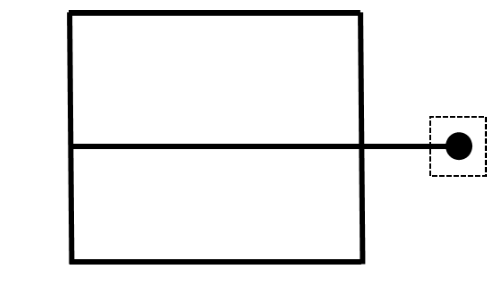
\includegraphics[width=0.5\columnwidth]{Figs/LatexImage3.png}
\end{figure}

\begin{enumerate}
     
   \item satellite’s altitude 
   \item satellite’s geometry  
   \item satellite’s atomic clocks 
   \item satellite’s velocity
\end{enumerate}

\item Which of the following is NOT a derivative of digital elevation model (DEM)?

\begin{enumerate}
\begin{multicols}{4}

    \item Slope 
   \item Aspect 
   \item Contour 
   \item Emissivity 
   \end{multicols}
\end{enumerate}

\item Which of the following is a core vector GIS operation?

\begin{enumerate}
    \item Overlaying 
   \item Contrast stretching 
   \item Histogram equalization 
   \item Band ratioing
\end{enumerate}

\item The wavelength at which maximum energy is radiated or emitted from the forest
fire at temperature of 700 °C is \rule{2cm}{0.15mm} (rounded off to one decimal place).

\item The standard error of a unit weight for a set of angle observations is 10\textquotedblright.
The minimum number of observations required to reduce the standard error of the
mean for this set of observations to 2\textquotedblright\ is  \rule{2cm}{0.15mm} \textit{(in integer)}.

\item  Which of the following is a core vector GIS operation?\\
      \ang{60;30;10} ± 10''\\  
      \ang{60;30;20} ± 20''\\
     The most probable value (MPV) of the angle is: 

\begin{enumerate}
\begin{multicols}{4}

    \item \ang{60;30;12} 
   \item \ang{60;30;15}  
   \item \ang{60;30;18} 
   \item \ang{60;30;14} 
   \end{multicols}
\end{enumerate}

\item In the figure, $d_1, d_2, d_3$ are three independently measured distances for estimating
the unknown distances $x$ and $y$. The correlation coefficient between the unknown
estimates approximately equals to  

\begin{figure}[H]
\centering
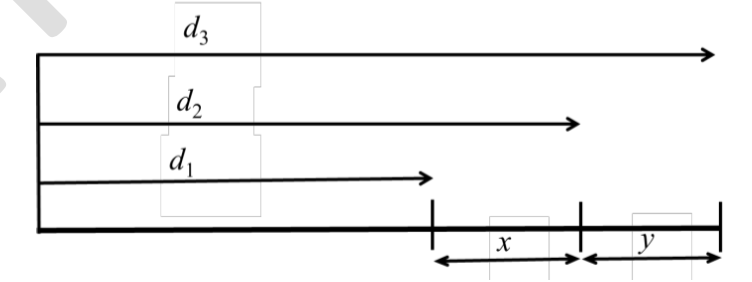
\includegraphics[width=0.5\columnwidth]{Figs/LatexImage4.png}
\end{figure} 

  $d_1$ = 100m ± 1cm\\ 
  $d_1$ = 150m ± 2cm \\
  $d_1$ = 175m ± 3cm 

  \begin{enumerate}
  \begin{multicols}{4}

    \item + 0.325 
   \item $-$ 0.496 
   \item + 0.755 
   \item $-$ 0.592
   \end{multicols}
  \end{enumerate}

\item Independent angles $AOB, BOC$ and $AOC$ were observed as shown in figure. The
standard error of all observations is same. The adjusted values of these angles
using the least squares adjustment are 

 \begin{figure}[H]
\centering
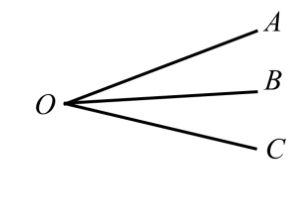
\includegraphics[width=0.5\columnwidth]{Figs/LatexImage5.png}
\end{figure}

  $AOB$ = \ang{30;00;20} \\
  $BOC$ = \ang{30;00;05}\\
  $AOC$ = \ang{60;00;10} 

  \begin{enumerate}
    \item $AOB$ = \ang{30;00;15} , $BOC$ = \ang{30;00;00}, $AOC$ = \ang{60;00;15} 
   \item $AOB$ = \ang{30;00;10} , $BOC$ = \ang{30;00;05}, $AOC$ = \ang{60;00;15} 
   \item $AOB$ = \ang{30;00;05} , $BOC$ = \ang{30;00;10}, $AOC$ = \ang{60;00;15} 
   \item $AOB$ = \ang{30;00;10} , $BOC$ = \ang{30;00;10}, $AOC$ = \ang{60;00;20}
  \end{enumerate}

\item To reduce the slope distance $(S)$ to an equivalent horizontal distance $(H)$ as shown in the figure given below, the following independent observations were taken.\\
  S = 29.95 m ± 0.01 m; $\theta = 4\degree 30' ± 10'$ . \\
  The required precision of computed horizontal distance is ± 0.005 m. Assume a “balanced accuracy” where the contribution to precision of the horizontal distance comes equally from the slope distance and angle measurements. The minimum number of angle observations to achieve the desired precision is\\ 
   (Given 1 radian = 206265 seconds) \\

   \begin{figure}[H]
\centering
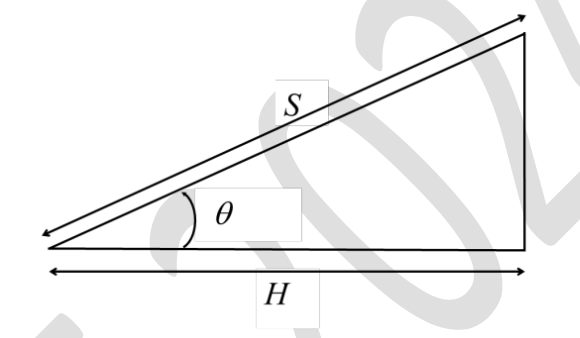
\includegraphics[width=0.5\columnwidth]{Figs/LatexImage6.png}
\end{figure} 
\begin{enumerate}
\begin{multicols}{4}

   \item 1 
   \item 2 
   \item 3 
   \item 4 
   \end{multicols}
  \end{enumerate}

\item Find the best match between remote sensing sensors (Column A) with their
characteristics (Column B)

\begin{table}[H]
         \centering
         \caption{}
         \begin{tabular}{|c|c|c|c|}
         \hline
              &Column A&  &ColumnB\\ \hline
              (P)& IRS LISS-III & (1) & 36 bands \\ \hline
              (Q)& Landsat TM& (2) & along track scanner\\ \hline
              (R)& Modis  & (3) & across track scanner \\ \hline
              (S)& Hyperion  & (4) & 18 bands \\ \hline 
               & & (5) & 242 bands\\ \hline
         \end{tabular}
         \label{tab:placeholder}
     \end{table}

\begin{enumerate}
    \item P\textemdash1, Q\textemdash5, R\textemdash2, S\textemdash3 
   \item P\textemdash3, Q\textemdash2, R\textemdash4, S\textemdash1 
   \item P\textemdash2, Q\textemdash3, R\textemdash1, S\textemdash5 
   \item P\textemdash1, Q\textemdash3, R\textemdash4, S\textemdash5
\end{enumerate}

\item Find the best match between Column A and Column B

\begin{table}[H]
         \centering
         \caption{}
         \begin{tabular}{|c|c|c|c|}
         \hline
              &Column A&  &ColumnB \\ \hline
              (P)& Radiant Flux& (1) & Dimensionless\\ \hline
              (Q)& Radiant Energy& (2) & Watts\\ \hline
              (R)& Radiant Exitance& (3) & Joules\\ \hline
              (S)& Reflectance& (4) & Watts $m^{-2}$\\ \hline 
              & & (5) & Watts $m^{-2}s^{-1}$\\ \hline
         \end{tabular}
         \label{tab:placeholder}
     \end{table}

\begin{enumerate}
    \item P\textemdash5, Q\textemdash4, R\textemdash3, S\textemdash1 
   \item P\textemdash5, Q\textemdash4, R\textemdash2, S\textemdash3 
   \item P\textemdash3, Q\textemdash1, R\textemdash2, S\textemdash4 
   \item P\textemdash2, Q\textemdash3, R\textemdash4, S\textemdash1

   
\end{enumerate}

\item Which of the following factors is/are responsible for ionospheric delay in GNSS
observations? 

\begin{enumerate}
    \item Total electron count in the ionosphere 
   \item Carrier signal frequency 
   \item Size of GPS receivers 
   \item Size and accuracy of atomic clocks
\end{enumerate}

\item Which of the following statements is/are CORRECT in the context of GPS data
collection methods?

\begin{enumerate}
  \item CORS (Continuously Operating Reference Station) can be used as a reference
(base) GPS receiver 
   \item Reference (base) receiver should record the observations for longer period as
compared to remote (rover) GPS receiver for applying corrections  
   \item Remote (rover) GPS receiver must always be placed on a known location for
applying the corrections of reference (base) GPS receiver 
   \item Reference (base) and remote (rover) GPS receivers must be placed on top of each
other for applying corrections
\end{enumerate}

\item Which of the following errors is/are corrected in Differential GPS (DGPS)?

\begin{enumerate}
   \item Tropospheric delays 
   \item Orbital errors 
   \item Ionospheric delays 
   \item Ambiguity in atomic clocks
\end{enumerate}


\item Which of the following statements is/are CORRECT?

\begin{enumerate}
    \item Network analysis can be done with vector data. 
   \item Linear features are clearly identified as discrete features in vector database. 
   \item Satellite images are in vector format. 
   \item Digital elevation model is in raster format.
\end{enumerate}

\item  In GIS, buffer is a zone with a specified width surrounding a spatial feature. Which
of the following statements regarding buffer is/are CORRECT?

\begin{enumerate}
    \item For a point feature, buffer is an ellipse with minor and major axes as buffer
distances 
   \item For a line feature, buffer is a band with a specified distance created around the line
conforming to the line’s curve 
   \item Buffer zones are polylines 
   \item For a polygon feature, buffer is a belt of a specified distance from the edge of the
polygon and conforming to its shape
\end{enumerate}

\item Which of the following statements about the Triangulated Irregular Network
(TIN) model is/are INCORRECT?
\begin{enumerate}
    \item TIN contains irregularly spaced sampled points 
   \item Triangulation is performed to form network of triangles. 
   \item In the TIN model, the edges represent features such as peaks and depression. 
   \item In the TIN model, the vertices represent features such as peaks and depression.
\end{enumerate}

\item  Which of the following statements is/are INCORRECT in the context of GIS? 

\begin{enumerate}
    \item CLIP erases a part of one of the input layers. 
   \item SPLIT overlays polygons and keeps all areas in both layers. 
   \item INTERSECT overlays polygons and keeps only the common portions of both layers. 
   \item UNION overlays polygons and keeps all areas in both layers.
\end{enumerate}

\item Which of the following is/are method(s) used for compact storage of raster GIS
data?
\begin{enumerate}
\begin{multicols}{4}

    \item Chain code 
   \item Run-length code 
   \item Quadtree 
   \item Decision-tree
   \end{multicols}
\end{enumerate}

\item Which of the following statements is/are CORRECT?
 \begin{enumerate}
     \item CARTOSAT-1 satellite can acquire across-track stereoscopic pairs of images of a
geographical region on the same day. 
   \item CARTOSAT-1 satellite can acquire across-track stereoscopic pairs of images of a
geographical region on successive days. 
   \item CARTOSAT-1 satellite can acquire along-track stereoscopic pairs of images of a
geographical region on the same day. 
   \item CARTOSAT-1 satellite can acquire along-track stereoscopic pairs of images of a
geographical region on successive days.
 \end{enumerate}



\item Which of the following statements is/are CORRECT for satellite image
interpretation?

\begin{enumerate}
    \item SWIR band is sensitive to moisture in soil and vegetation 
   \item Blue band is not useful to discriminate between water and snow 
   \item NIR band is useful to discriminate between land and water 
   \item Green band is useful to discriminate between cloud and snow 
\end{enumerate}

\item Which of the following CANNOT be used as visual interpretation key(s) for
satellite images?

\begin{enumerate}
\begin{multicols}{4}

    \item Texture 
   \item Projection 
   \item Pattern 
   \item Association 
   \end{multicols}
\end{enumerate}
    
\item Which of the following parts of the electromagnetic spectrum is/are used in
satellite remote sensing for earth observation? 

\begin{enumerate}
    \item Visible wavelengths 
   \item Thermal Infrared wavelengths 
   \item Radio wavelengths 
   \item Gamma wavelengths
\end{enumerate}

\item Using the following data, the spatial resolution of a push-broom sensor
is \rule{2cm}{0.15mm} m \textit{(in integer)}.

    \textbf{Data:}\\
   Orbital altitude (above earth surface) = 1000 km\\
  Number of spectral bands = 5\\
  Number of detectors/CCDs (charged coupled devices) in a row = 4000\\
  Ground swath = 20 km\\

\item If the plotting accuracy of a map is 0.25 mm and the scale of the same map is
1:100000, what will be the minimum ground distance that can be plotted on the
map? 

\begin{enumerate}
\begin{multicols}{4}

    \item 2.5 m 
   \item 25 m 
   \item 250 m 
   \item 2500
   \end{multicols}
\end{enumerate}

\item The Survey of India toposheet number 43$\frac{D}{6}$

\begin{enumerate}
\begin{multicols}{4}

    \item 1° by 1° 
   \item 25' by 25' 
   \item 15' by 15' 
   \item 7.5' by 7.5'
\end{multicols}
\end{enumerate}

\item Universal Transverse Mercator (UTM) is a

\begin{enumerate}
    \item conical projection 
   \item azimuthal projection 
   \item azimuthal projection 
   \item cylindrical projection
\end{enumerate}

\item Change Point (CP) in levelling refers to a location where

\begin{enumerate}
    \item only backsight reading is taken 
   \item both backsight and foresight readings are taken 
   \item survey work ends 
   \item staff reading is taken on a benchmark
\end{enumerate}

\item  1 At a fixed instrument location in levelling, if the backsight reading at a point P is
more than the foresight reading at a point Q, then

\begin{enumerate}
    \item point P has lower elevation than point Q 
   \item point P has higher elevation than point Q 
   \item the elevation difference between P and Q depends on height of the instrument 
   \item the elevation difference between P and Q depends on benchmark elevation
\end{enumerate}

\item ``Transit the telescope'' of a theodolite involves

\begin{enumerate}
     \item rotating the theodolite about its vertical axis 
   \item rotating the telescope about its trunnion axis 
   \item rotating the telescope about its line of collimation 
   \item rotating the theodolite by 90° in horizontal plane
\end{enumerate}

\item Scale of a vertical aerial photograph of an undulating terrain is

\begin{enumerate}
    \item directly proportional to the height of terrain 
   \item inversely proportional to the focal length of camera lens 
   \item directly proportional to the flying height of aircraft 
   \item uniform throughout the photograph
\end{enumerate}

\item  Isocentre of a tilted photograph is
\begin{enumerate}
    \item intersection of the optical axis of the aerial camera with the plane of the photograph 
   \item the point of aerial photograph where a plumb line dropped from exposure station pierces the photograph 
   \item angle of tilt of the photograph 
   \item the point on the photograph where the bisector of the angle of tilt meets the
photograph 
\end{enumerate}

\item The magnetic bearing of a line in the year 1990 was found to be N 40°30' W and
magnetic declination was 3°30' E. If the present magnetic declination is 2°10' W,
the magnetic bearing now (in reduced bearing system) would be 

\begin{enumerate}
\begin{multicols}{4}

 \item S 30°50' W 
   \item N 30°50' W 
   \item S 34°50' W 
   \item N 34°50' W
   \end{multicols}
\end{enumerate}

\item Map (A) represents all the roads, street lights, trees and buildings of a campus of
5 ${km}^2$. Another map (B) represents the forest and agricultural area of a district of
10000 ${km}^2$. Considering the physical size of both the maps (A) \  (B) same, which
of the following statements is/are CORRECT?

\begin{enumerate}
    \item Map (A) is at relatively large scale 
   \item Map (B) is at relatively large scale 
   \item Both maps are at same scale 
   \item Both maps are not at same scale 
\end{enumerate}

\item Which of the following statements is/are CORRECT? 
\begin{enumerate}
    \item Triangulation is preferred in plain areas, whereas trilateration is preferred in hilly
areas 
   \item Triangulation is preferred in hilly areas, whereas trilateration is preferred in plain
areas 
   \item In triangulation, the angles are measured with greater accuracy, while in
trilateration, sides are measured with greater accuracy 
   \item In trilateration, the angles are measured with greater accuracy, while in
triangulation, sides of triangles are measured with greater accuracy 
\end{enumerate}

\item Which of the following statements is/are CORRECT?

\begin{enumerate}
    \item Bowditch rule in traverse adjustment is particularly useful, where angular and linear
measurements are equally precise 
   \item Transit rule in traverse adjustment is particularly useful, where angular
measurements are more precise than linear measurements 
   \item In Bowditch rule, the traverse adjustment is done using arithmetic sum of latitudes
or departures of the traverse 
   \item In Transit rule, the traverse adjustment is done using perimeter of the traverse
\end{enumerate}

\item  Consider a point A on the surface of Earth, its elevation with respect to EGM2008
(geoid) is 95.5 m. The geoidal undulation at point A is 4.5 m. The orthometric height
of point A is \rule{2cm}{0.15mm} m (rounded off to one decimal place).

\item If the longitudinal overlap in aerial photographs is kept as 65\%, the common overlap
(superlap) between three successive photographs is \rule{2cm}{0.15mm}\% \textit{(in integer)}. 

\item The Representative Fraction (RF) of the graphical scale given below is 1/X, where X is \rule{2cm}{0.15mm}($in$ $integer$). //

\begin{figure}[H]
\centering
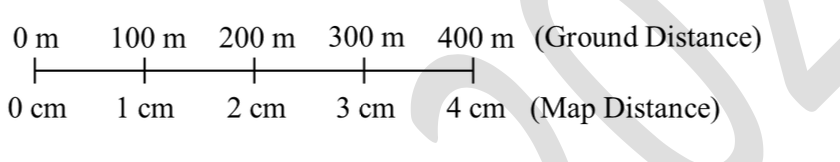
\includegraphics[width=0.5\columnwidth]{Figs/LatexImage7.png}
\end{figure}

\item The combined correction for curvature of Earth and refraction in levelling for a
distance of 6 km would be \rule{2cm}{0.15mm}m \textit{(rounded off to two decimal places)}.\\ 
   Assume the radius of earth is 6370 km.

\item In tangential method of tacheometry, two vanes in a staff were fixed at a distance
of 1.0 m with the bottom vane fixed at 1.0 m. The levelling staff was held vertical
at a point P and the vertical angles of the vanes observed were 5°30' and 3°15',
respectively. The vertical distance between the instrument axis and the bottom vane
would be \rule{2cm}{0.15mm} \textit{(rounded off to two decimal places)} 

\item A line measures 15 cm on an aerial photograph, while it measures 5 cm on a map
at 1:24000 scale. The photograph was taken using a camera lens of 20 cm focal
length. Average elevation of terrain is 240 m above mean sea level. The flying
height of the aircraft above mean sea level is\rule{2cm}{0.15mm} m \textit{(in integer)}.

\item A high tower appeared on an aerial photograph taken at 1000 m above mean sea
level with a camera lens of 15 cm focal length. The radial distances of the top and
bottom images of the tower from principal point of photograph are 92.6 mm and
78.3 mm, respectively. If the average elevation of terrain is 300 m above mean sea
level, then the height of the tower above ground is \rule{2cm}{0.15mm} m \textit{(rounded off to the nearest integer)}

\item A four-band multispectral image of size 64 × 64 pixels has 560 header bytes. The
per pixel depth of the image is 2 bytes. The total number of bytes required to store
this image on the disk in the Band Interleaved by Line (BIL) format will be  
\begin{enumerate}
\begin{multicols}{4}

    \item 33328 
   \item 32338 
   \item 33823 
   \item 33283
   \end{multicols}
\end{enumerate}

\item A one-dimensional normalized kernel $ \frac{1}{4} [\begin{smallmatrix}1   2   1\\ \end{smallmatrix} ] $ is convolved with an image to produce an intermediate result. The intermediate image of this operation is again convolved with the same kernel to produce a final result. The equivalent kernel to achieve the same final result in one step from the original image is given as

\begin{enumerate}
\begin{multicols}{4}

  \item $ \frac{1}{16}[\begin{smallmatrix}1   4   6 4 1\\ \end{smallmatrix} ] $ 
   \item $ \frac{1}{16}[ \begin{smallmatrix}1   2   1 2 1\\ \end{smallmatrix} ] $ 
   \item $ \frac{1}{8}[ \begin{smallmatrix}1   2   4 2 1\\ \end{smallmatrix} ] $ 
   \item $ \frac{1}{10}[ \begin{smallmatrix}1   2   4 2 1\\ \end{smallmatrix} ] $
   \end{multicols}
\end{enumerate}

\item The histogram equalization applied to a digital image generally DOES NOT yield
a truly uniform histogram of the transformed image due to

\begin{enumerate}
    \item discrete nature of pixel values 
   \item poor contrast of the original image 
   \item low frequency image information 
   \item presence of edges
\end{enumerate}


\item Which type of contrast stretching is represented by the following figure?  \\

\begin{figure}[H]
\centering
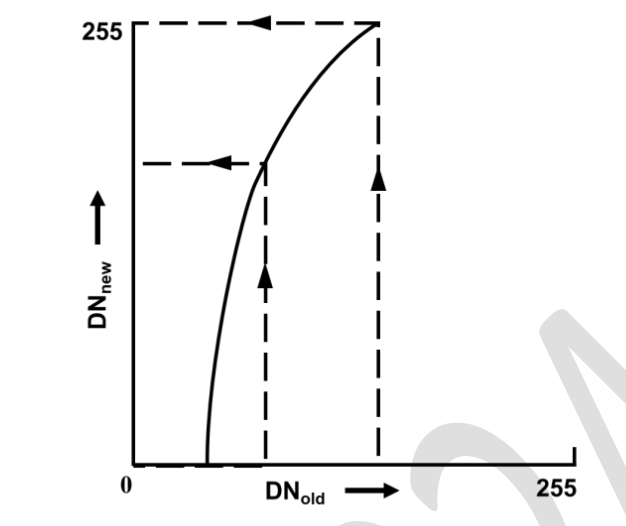
\includegraphics[width=0.5\columnwidth]{Figs/LatexImage8.png}
\end{figure}  

\begin{enumerate}
    \item Linear contrast stretch 
   \item Multiple linear stretch 
   \item Logarithmic stretch 
   \item Gaussian stretch
\end{enumerate}

\item Contrast enhancement is a type of \rule{2cm}{0.15mm} enhancement.
\begin{enumerate}
\begin{multicols}{4}

    \item spectral 
   \item spatial 
   \item radiometric 
   \item temporal
   \end{multicols}
\end{enumerate}

\item \rule{2cm}{0.15mm} is a raster image resampling technique that DOES NOT alter any of the
output cell values from the input raster dataset.  

\begin{enumerate}
\begin{multicols}{4}

 \item Nearest neighbor 
   \item Cubic convolution 
   \item Bilinear 
   \item Kriging
   \end{multicols}
\end{enumerate}

\item De-stripping in radiometric correction is used to correct a type of 

\begin{enumerate}
\begin{multicols}{4}

    \item sensor defect 
   \item atmospheric effect 
   \item path radiance 
   \item geometric error
   \end{multicols}
\end{enumerate}

\item The figure given below shows the Fourier spectrum obtained by applying filter on
a remote sensing image in frequency domain. Zone A represents the location of
\rule{2cm}{0.15mm} components. \\
\begin{figure}[H]
\centering
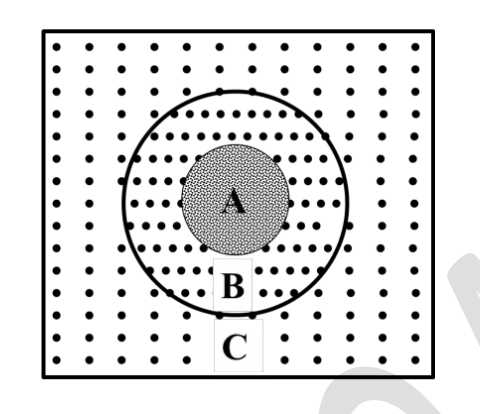
\includegraphics[width=0.5\columnwidth]{Figs/LatexImage9.png}
\end{figure} 

 \begin{enumerate}


    \item low frequency 
   \item mid frequency 
   \item mid to high frequency 
   \item high frequency
   
      \end{enumerate}

\item For the following covariance matrix ($\Sigma$) of a multispectral image, which of the
statements is/are INCORRECT?\\

\begin{figure}[H]
\centering
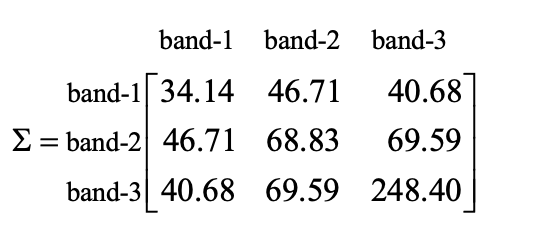
\includegraphics[width=0.5\columnwidth]{Figs/LatexImage10.png}
\end{figure} 

\begin{enumerate}
   \item band-1 and band-2 have maximum correlation 
   \item band-2 and band-3 are least correlated 
   \item band-3 conveys the maximum information content 
   \item band-1 conveys the minimum information content 
\end{enumerate}

\item Which of the following statistical measures CANNOT be computed from the
multispectral image histograms?

\begin{enumerate}
    \item Mean, skewness, kurtosis 
   \item Covariance matrix 
   \item Co-occurrence matrix 
   \item Correlation matrix 
\end{enumerate}

\item Which of the following statements about Principal Component Analysis (PCA)
is/are CORRECT?

\begin{enumerate}
     \item A two-dimensional data set can have up to four principal components. 
   \item The first principal component accounts for the majority of conceivable data
variation. 
   \item The second principal component attempts to encapsulate the mode of the data. 
   \item The transformed principal components are linear combinations of the original
variables and are orthogonal.
\end{enumerate}

\item In the context of satellite image classification, which of the following statements
is/are CORRECT? 
\begin{enumerate}
    \item Both ANN and Fuzzy C-means clustering are parametric classifiers 
   \item Both ANN and Fuzzy C-means clustering are non-parametric classifiers 
   \item ANN can be both supervised and unsupervised classification method 
   \item Fuzzy C-means clustering is a supervised classification method
\end{enumerate}

\item Which of the following filters can be used to suppress the low frequency component
of a raster image? \\

\begin{figure}[H]
\centering
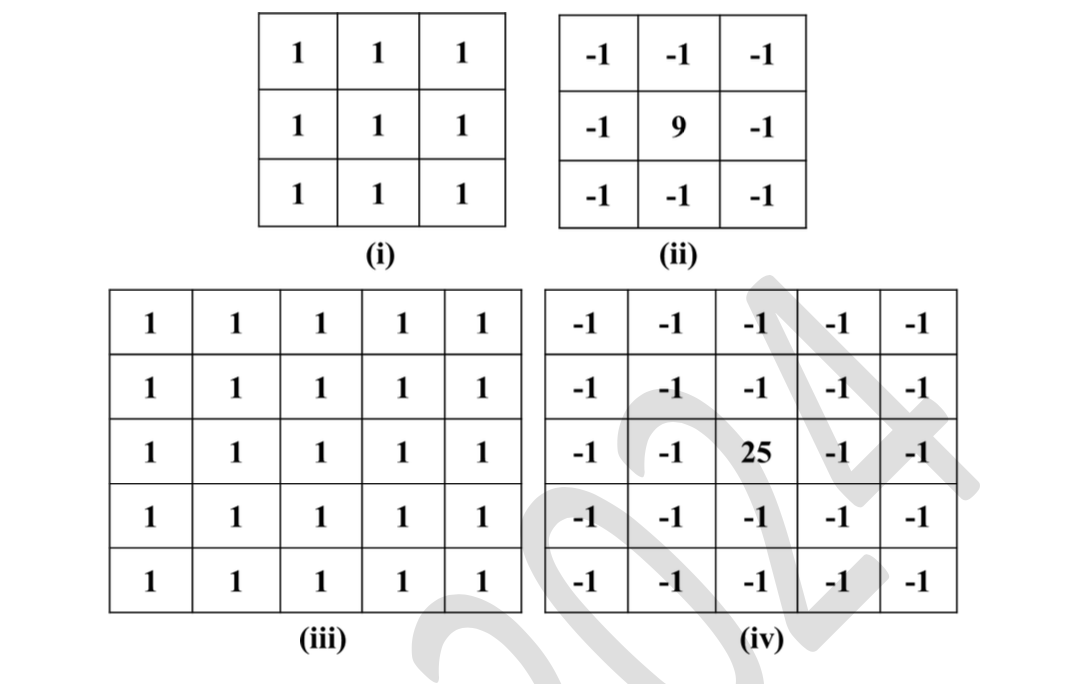
\includegraphics[width=0.5\columnwidth]{Figs/LatexImage11.png}
\end{figure} 

 \begin{enumerate}
 \begin{multicols}{4}

     \item(i) 
   \item (ii) 
   \item (iii) 
   \item (iv)
   \end{multicols}
 \end{enumerate}

\item Which of the following statements about image ratio is/are CORRECT?]\\


\begin{enumerate}
    \item It cannot be used to suppress the effects of topography 
   \item It cannot be used to suppress the effects of differential sun-illumination 
   \item It helps in suppressing the effects of differential sun-illumination 
   \item It helps in suppressing the effects of topography 
\end{enumerate}

\item Which of the following statistical classification algorithms is/are represented by the
figure given below?\\

\begin{figure}[H]
\centering
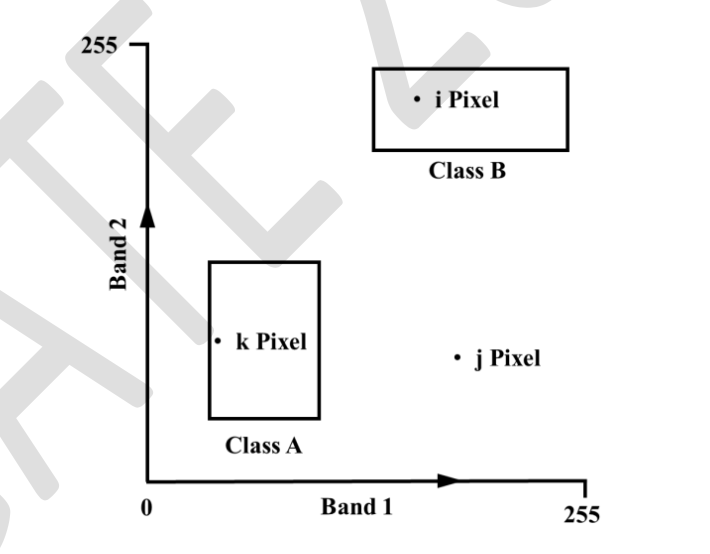
\includegraphics[width=0.5\columnwidth]{Figs/LatexImage12.png}
\end{figure} 

\begin{enumerate}
    \item Minimum distance to mean classification 
   \item Parallelepiped classification 
   \item Maximum likelihood classification 
   \item k-means clustering 
\end{enumerate}

\item Using the given 3 × 3 pixel kernel and original image and applying the concept of
convolution, the value of central pixel of the output image is \rule{2cm}{0.15mm} \textit{(in integer)}

\begin{figure}[H]
\centering
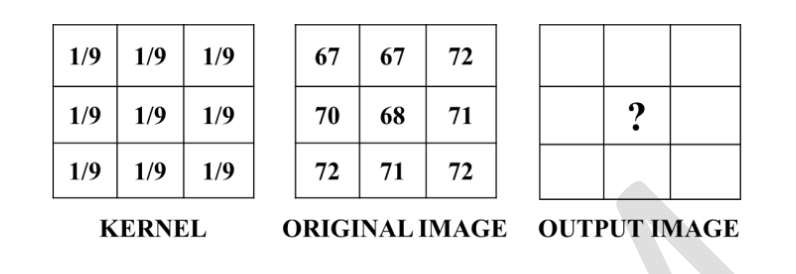
\includegraphics[width=0.5\columnwidth]{Figs/LatexImage13.png}
\end{figure}

\item A four-band multispectral image with pixel size of 50 m × 50 m covers a ground
area of 20 km × 20 km. If the radiometric resolution of the satellite data is 8 bits,
then the uncompressed satellite image contains\rule{2cm}{0.15mm}  kilobytes (kB) of data \textit{(in integer)}.

\item In spatial interpolation using coordinate transformations for image-to-map
rectification, the minimum number of ground control points (GCPs) required to
perform a third-order transformation is \rule{2cm}{0.15mm}($in$ $integer$). 

\item In an image with 6-bit quantization level, the pixel values of a scene are between 25
and 55. A linear contrast stretch is applied to the image covering the full dynamic
range. A pixel value 40 in the original image will be mapped to \rule{2cm}{0.15mm} \textit{(rounded off to nearest integer)} in the stretched image.







\end{enumerate}
\end{document}

